% !TEX root = ../../../main.tex
% 来源：高中物理甲种本·第二册（热学·电学）
% 章节：固体和液体的性质 / 空间点阵
% 原始文件：4.tex，行 121-133
% 类型：tikz
% ---
	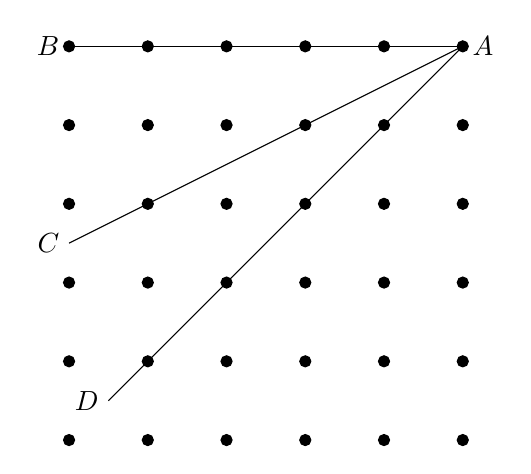
\begin{tikzpicture}[>=stealth, scale=1 ]

\foreach \x in {0,1,2,...,5}
\foreach \y in {0,1,2,...,5}
{
\draw [fill=black](\x,\y) circle (2pt);
}

\draw(0,5)node [left]{$B$}--(5,5)node [right]{$A$};
\draw (5,5)--(0,3-.5)node [left]{$C$};
\draw (5,5)--(.5,.5)node [left]{$D$};

\end{tikzpicture}
